% Hier können die einzelnen Kapitel inkludiert werden. Sie müssen in den 
% entsprechenden .TEX-Dateien vorliegen. Die Dateinamen können natürlich 
% angepasst werden.

\section{Einleitung}
\label{sec:Einleitung}
Für viele Menschen stellt das Internet in der heutigen Zeit das wichtigste
Medium zur Informationsgewinnung dar. Durch die Entwicklung des Internets hin
zum Web 2.0 werden dem Nutzer immer neue Möglichkeiten geboten, auf das
umfassende Angebot an Informationen im Internet zuzugreifen. Der Zugriff auf
dieses Informationsangebot gestaltet sich hierbei zunehmend interaktiver.
Diese Interaktivität wird immer häufiger auch von Unternehmen genutzt.
Unternehmen präsentieren sich nicht mehr nur auf der firmeneigenen
Internetseite, sondern betreiben Marketing in sozialen Netzwerken,
veröffentlichen Neuigkeiten in Blogs und aquirieren neue Mitarbeiter über
Internetplatformen. Der Trend hin zur Nutzung dieser modernen
Kommunikationsmittel zeigt, dass es hiermit möglich ist weltweit eine große
Zielgruppe anzusprechen und auf sich aufmerksam machen zu können.

Im Rahmen des Projektes "`Virtueller Campus Lingen"' sollen diese neuen
Möglichkeiten der Internetpräsenz auch für den Standort Lingen der Hochschule
Osnabück nutzbar gemacht werden. Hierbei soll der neue Campus des
Studienstandorts Lingen einer breiten Masse an Studieninteressierten
präsentiert werden.

Bei der Durchführung eines Projektes von diesem Ausmaß ist es wichtig die
Komplexität handhabbar zu machen und das Projekt möglichst genau zu planen,
steuern und kontrollieren zu können. In dieser Ausarbeitung soll aus diesem
Grund die Vorgehensweise bei der Auftragsfindung, der Konzeptionierung,
Umsetzung und Reflexion des Projektes "`Virtueller Campus Lingen"' aus Sicht der
Unternehmensführung dargestellt werden. Zunächst wird im Abschnitt
"`Projektauftrag"' die Projektidee, sowie das Projektumfeld und die Projektziele
herausgestellt. In den Projektzielen wird hierbei der Nutzen des Projektes
für den Auftraggeber verdeutlicht. Auf den Projektautrag aufbauend soll
die Entwicklung des Projektkonzeptes im Abschnitt "`Konzeptionierung"'
beschrieben werden. Nachfolgend werden die für die Umsetzung des Projektes
benötigten Ressourcen Zeit und Kosten geplant. Anschließend werden im Abschnitt
"`Projektdurchführung"' sowohl die Organisation der Projektgruppe als auch die
einzelnen Phasen, in denen das Projekt durchgeführt wurde, erläutert.  

In der darauffolgenden Projektreflexion werden geplante und benötigte Ressourcen
in einem Soll-Ist-Vergleich gegenübergestellt und die Erreichung der zuvor
aufgestellten Projektziele verifiziert. Für den Auftraggeber werden hier die
angefallenen Kosten den erreichten Projektzielen und somit dem Nutzen des
Projektes gegenübergestellt. Weiterhin werden die subjektiven Eindrücke der
Projektmitglieder im Bezug auf die Kommunikation, das Verhalten in der Gruppe
und die Betreuuung der Arbeit durch die Dozenten reflektiert. Nach der
Reflektion wird ein Ausblick auf eine mögliche Weiterführung des Projektes
gegeben. Abschließend wird von der Projektgruppe eine Handlungsempfehlung
bezüglich der Veröffentlichung und Erweiterung des Projektes an den Auftraggeber
ausgesprochen.
\section{Projektauftrag}
\label{sec:Projektauftrag}

\subsection{Projektidee}
\label{sec:Projektidee}

Um diesen neuen Studienstandort auch möglichst vielen Studieninteressierten
bekannt zu machen haben sich die Mitglieder des Projektes "`Virtueller Campus
Lingen"' dazu eintschieden eine Maßnahme zur Außendarstellung des Campus zu
entwickeln. Hierzu sollen modere Technologien des Internets verwendet werden, um
die junge Zielgruppe des Studieninteressierten direkt anzusprechen. Ein
besonderes Augenmerk soll hierbei auf eine visuelle Darstellung gelegt werden,
um den Studieninteressierten auf möglichst ansprechende und interessante Art und
Weise ein Bild vom Campus Lingen zu vermitteln.

% TODO: Auch auf Messen präsentieren?
\subsection{Projektumfeld}
\label{sec:Projektumfeld}

% TODO: Umsetzung durch Projektteam, jedoch nicht die einzigen Beteiligten
% TODO: Referrenz auf Stakeholderanalyse
% TODO: Projektgruppen nennen und Besonderheiten herausstellen

Nachdem geklärt wurde, auf welche Weise das Projekt realisiert werden soll,
sollen nachfolgend alle Stakeholder, die an dem Projekt "`Virtueller Campus
Lingen"' beteiligt sind und deren Aufgaben im Projekt, herausgestellt werden.
Das Projektteam, welches aus Andreas Makeev, Raphael Otten, Carsten Sandker und
Jannik Fangmann besteht, stellt hierbei nur einen Teil der Stakeholder dar.
Dieser Teil der Stakeholder agiert als Entwickler und ist für die Umsetzung der
Projektidee zuständig. Neben den Entwicklern sind weitere Personen oder
Personengruppen an dem Projekt beteiligt, die die Rollen "`Betreuer"',
"`Aufraggeber"', "`Berater"' und "`Anwender"' in dem Projekt übernehmen.

Wie bereits herausgestellt ist der Projektinhalt die Visualisierung des Campus
Lingen. An diesem Standort der Hochschule Osnabrück ist die Fakultät
Management, Kultur und Technik ansässig. Aus diesem Grund nimmt die Leitung
dieser Fakultät auch die Rolle des Auftraggebers im Projekt ein. Die
Fakultätsleitung besteht hierbei aus dem Dekan der Fakultät, Prof. Dr. Frank
Blümel, und den Leitern der vier Institute aus denen die Fakultät besteht.
Diese sind Prof. Dr. Michael Ryba für das Institut Management und Technik,
Prof. Dr.-Ing. Wolfgang Arens-Fischer für das Institut für Duale Studiengänge,
Prof. Dr. Dagmar Schütte für das Institut für Kommunikationsmanagement und
Prof. Dr. Bernd Ruping für das Institut für Theaterpädagogik.

Die Rolle der Betreuer wird hierbei von den Projektpaten Stefan Feldker und
Prof. Dr. Ralf Westerbusch übernommen. Diese sollen der Projektgruppe bei
Fragen zur Seite stehen und diese durch den Prozess der Projektumsetzung
begleiten. Weiterhin stellen sie die Zwischenstation bei der Kommunikation der
Entwickler mit der Fakultätsleitung dar.

Auch der Datenschutzbeauftragte der Hochschule Osnabrück, Prof. Dr. Alfred
Scheerhorn ist am Projekt beteiligt. Das Projekt soll, wie bereits
herausgestellt, im Stile von Google Street View realisiert werden. Hierbei
sollen die Benutzer durch 360-Grad Fotos des Campus navigieren. Die Umsetzung
des Projektes beinhaltet also auch die Veröffentlichung dieser Fotos im
Internet. Bei den datenschutzrechtlichen Fragen, die sich hieraus ergeben, soll
Herr Scheerhorn dem Projektteam als Berater zur Seite stehen.

Neben den bereits erwähnten Personen und Personengruppen gehören auch die
Benutzer der zu realisierenden Anwendung zu den Stakeholdern des Projektes.
Alle Stakeholder, die an dem Projekt beteiligt sind, sind in Abbildung X
% TODO: Verweis auf Anhang
dargestellt.

\subsection{Projektzielsetzung}
\label{sec:Projektzielsetzung}

Die Projektzielsetzung stellt einen wichtigen Punkt der Projektplanung dar.
Durch die Projektzielsetzung soll eine gemeinsame Zielvorstellung entwickelt
werden, welche verbindlich festgehalten wird.\footnote{\citet[S.~34]{litke2007}}
Diese Ziele müssen mit dem Auftraggeber abgestimmt und von den Entwicklern im
Laufe des Projektes umgesetzt werden. Nur bei Erreichung der Projektziele kann
das Projekt als erfolgreich abgeschlossen bezeichnet werden. Die Zielerreichung
wird hierbei nach Abschluss des Projektes untersucht.

Ein Zielsystem, das für das vorliegende Projekt erstellt wurde, stellt alle 
Ziele des Projektes übersichtlich dar und ist in \anhang{Zielsystem} abgebildet. 
Der bereits in\verweis{Projektidee} definierte Projektauftrag stellt das Hauptziel, 
das Projektziel in der obersten Ebene, dar. Das Hauptziel des Projektes ist:

\begin{quote}
Konzeptionierung und Entwicklung einer Anwendung zur Darstellung des 
Campus Lingen als attraktiven Studienstandort.
\end{quote}

Um dieses sehr allgemein formulierte Hauptziel zu operationalisieren, wird
es in folgende sechs Oberziele zerlegt:

\begin{itemize}
  \item Außendarstellung des Campus Lingen verbessern
  \item Kosten gering halten / Finanzierung sichern
  \item Campus vollständig und realistisch abbilden
  \item Nachhaltigkeit sichern
  \item Zielgruppe junger Studieninteressierter direkt ansprechen
  \item Qualität des Internetauftritts erhalten
\end{itemize}

In diesen Oberzielen spiegelt sich das Hauptziel des Projektes wider. Die
sechs Oberziele bieten jedoch noch nicht den gewünschten Grad der
Operationalisierung. Aus diesem Grund werden die einzelnen Oberziele ebenfalls
in mehre Unterziele zerlegt. Die Unterziele sind in \anhang{Zielkatalog}
dargestellt.

Diese Ziele sind nicht mehr durch andere Ziele beschreibbar und 
ihnen können konkrete Maßnahmen zur Erreichung zugeordnet werden. Zusätzlich sind die
Ergebnisse dieser Ziele messbar und machen die Erreichung des Oberziels und
somit schließlich die Erreichung des Hauptziels bewertbar. Um die Relevanz der
einzelnen Unterziele zu verdeutlichen und Missverständnisse bezüglich dieser
Relevanz zu vermeiden, werden diese in die Kategorien \textbf{Muss}-, \textbf{Soll}-, und
\textbf{Kann}-Ziele eingeordnet. 
Muss-Ziele sind hierbei elementar für die
Fertigstellung und den Erfolg des Projektes. Sollten diese Ziele nicht erfüllt
sein, kann das Projekt nicht erfolgreich abgeschlossen werden. Das Nichterfüllen von Soll-Zielen führt
hingegen nicht sofort zum Scheitern des Projektes. Das Endprodukt wird jedoch
stark in seinen Funktionen eingeschränkt sein. Die Erfüllung von Kann-Zielen
steigert nur den Wert des Projektes. Eine Erfüllung dieser Ziele ist nicht
zwingend erforderlich.

Die Muss- Soll- und Kann-Ziele werden im Zielsystem durch eine Ampeldarstellung
abgebildet. Muss-Ziele wurden im Zielsystem rot , Soll-Ziele gelb und 
Kann-Ziele grün hervorgehoben.

Neben der Unterteilung in Muss-, Kann- und Soll-Ziele wurden die Ziele auf der
untersten Ebene weiterhin in die Kategorien "`Sachziele"' und
"`Betriebswirtschaftliche Ziele"' eingeteilt. Die betriebswirtschaftlichen
Ziele repräsentieren hierbei besonders die Interessen der Auftraggeber. Durch
die Sachziele wird hingegen der angestrebte Funktionsumfang der Anwendung
verdeutlicht.

Eine abschließende Differenzierung der Ziele wird durch die Unterteilung 
in qualitative und quantitative Ziele gegeben. Diese Unterteilung ist wichtig
für die spätere Verifikation der Zielerreichung, denn nur die Erreichung von quantitativen
Zielen lässt sich durch Zielindikatoren bestimmen und verifizieren. 
Für qualititative Ziele lassen sich dagegen keine Zielindikatoren
finden, da diese einen Zielzustand beschreiben, der nur subjektiv wahrgenommen werden kann.
Zur Verifikation der Projektziele werden aus diesem Grund nur die quantitativen Ziele betrachtet.

Alle operationaliserten Ziele werden mit einem entsprechenden Zielindikator, der die Erreichung dieses
Ziel verifiziert, in \anhang{Zielkatalog} vorgestellt.
\section{Konzeptionierung}
\label{sec:Konzeptionierung}

An den Zielen des Projektes \acs{VCL} wird deutlich, dass eine visuelle und
attraktive Darstellung des Campus Lingen entwickelt werden muss. Auf welche Art
und Weise die Realisierung des Projektziels konkret erfolgen soll, ist jedoch in
der Projektzielsetzung nicht festgelegt. Aus diesem Grund wird in der
Konzeptionierungsphase von der Projektgruppe ein Konzept für ein System
entwickelt, mit dem die zuvor definierten Ziele erreicht werden können. Die
Konzeptionierungsphase kann hierbei in die Erstellung des Grobkonzeptes, die
iterative Erarbeitung des Feinkonzeptes und die abschließende Festlegung des
Feinkonzeptes unterteilt werden. Der Ablauf der drei Teilphasen wird im
Folgenden näher erläutert.

\subsection{Grobkonzept}
\label{sec:Grobkonzept}

Das Ziel einer möglichst ansprechenden, visuellen Darstellung des
Studienstandorts Lingen und des neuen Campus unter Verwendung moderner
Webtechnologien lässt sich auf verschiedenste Weisen realisieren. 

In einem Ideenfindungsprozess hat die Projektgruppe für die Erreichung der
Projektziele geeignete Umsetzungsmöglichkeiten identifiziert. Mit der
Brainstorming-Methode werden zunächst sämtliche Ideen zur Realisierung der
Projektidee gesammelt. Die Ideensammlung, die auf diese Weise entstand, wird
anschließend gefiltert und sortiert. Die einzelnen Ideen werden zu Clustern, wie
beispielsweise "`Anforderungen aus dem Zielsystem"', "`Technologien"' und
"`Funktionalität des Systems"' zusammengefasst. Anhand dieser strukturierten
Ideensammlung werden dann konkrete Möglichkeiten zur Umsetzung der Projektidee
herausgearbeitet. Nach einer ersten Filterung der Umsetzungsmöglichkeiten hat
sich die Projektgruppe auf die folgenden drei Realiserungsalternativen geeinigt. 

\begin{description}
\item[Fotogalerie] \hfill \\
Innerhalb einer Fotogalerie soll dem Anwender der modernisierte Studienstandort
Lingen näher gebracht werden. Zu den Fotos könnten entsprechende
Informationstexte, Beschreibungen und weiterführende Links für
Studieninteressierte hinterlegt werden.

\item[Virtueller Rundgang im Stile von Google Street View] \hfill \\
Der Anwender soll interaktiv durch Panoramafotos von den Räumlichkeiten des
Campus navigieren können. Auch bei dieser Möglichkeit der Projektrealisierung
könnten dem Nutzer weiterführende Informationen zu den abgebildeten Inhalten
präsentiert werden.

\item[Virtueller Rundgang durch ein 3D-Modell] \hfill \\
Bei dieser Möglichkeit der Umsetzug soll ein 3D-Modell des gesamten
Campusgebäudes erstellt werden. Der Nutzer könnte dann virtuell duch die
modellierten Räumlichkeiten des Campus navigieren und auf diese Weise einen
Eindruck vom Studienstandort erlangen.
\end{description}

Hierbei unterscheiden sich die einzelnen Alternativen in Innovativität,
Attraktivität für den Anwender, Komplexität der Umsetzung und Grad der Zielerreichung voneinander.
Die folgende \tabelle{AlternativenVergleich} stellt die drei Varianten
hinsichtlicher der vier genannten Kritierien gegenüber.

% \begin{table}[h]
% \centering
% 
% \caption{Soll-Ist-Vergleich der Kostenplanung}%
% \label{tab:AlternativenVergleich}%
% \end{table}

\tabelleEinfg{Soll-Ist-Vergleich der Kostenplanung}{tab:AlternativenVergleich}{AlternativenVergleich}

Die vorangegangene Tabelle stellt die drei möglichen Lösungsansätze mit den Kriterien 
Innovativität, Attraktivität, Komplexität und dem Grad der Zielerreichung dar. Die 
Fotogalerie hat im Gegensatz zu den anderen Ansätzen eine geringe Innovativität. Dies 
resultiert daraus, dass eine statische Fotogalerie im Vergleich zu virtuellen Rundgängen 
innovationslos ist. Die Fotogalerie erreicht somit nur eine mittlere Attraktivität. Die 
beiden anderen Lösungsansätze besitzen aufgrund der hohen Innovativität ebenfalls eine hohe 
Attraktivität. Die Komplexität der 3D-Modellierung und des virtuellen Rundgangs sind dagegen 
höher als die der Fotogalerie, da der Einarbeitungsaufwand bei diesen beiden Ansätzen höher 
und langwieriger ist. Die Fotogalerie hat im Vergleich zu den anderen Lösungsansätzen nur 
einen geringen Grad der Zielerreichung. Die 3D-Modellierung und der virtuelle Rundgang erreichen 
hingegen einen hohen Grad der Zielerreichung, da die junge Zielgruppe durch innovative und attraktive Ansätze
effektiver angesprochen wird.

% Die Projektgruppe geht davon aus, dass vielen Nutzern innerhalb der Zielgruppe
% diese Darstellungsform durch Google Street View bereits bekannt ist. Um von den
% vorhandenen Erfahrungen der Nutzer profitieren zu können sollen bekannten
% Steuerungselemente von Google Street View adaptiert werden. Diese sind in
% \abbildung{GoogleStreetView} dargestellt.

% \begin{figure}[htb] 
% \centering
% 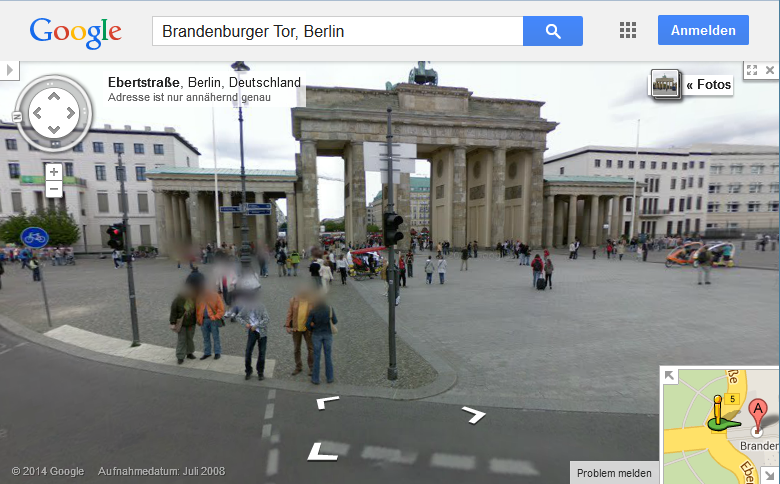
\includegraphics[width=0.7\textwidth]{GoogleStreetView.png}
% \caption[Google Street View]{Google Street View\protect\footnotemark}
% \label{fig:GoogleStreetView}
% \end{figure}
% \footnotetext{Screenshot von \url{https://maps.google.de/}}

% Die Realisierung der Projektziele wäre nach einer ersten Einschätzung der
% Projektmitglieder mit jeder der dei vorgestellten Umsetzungsmöglichkeiten
% vorstellbar. Im weiteren Verlauf der Konzeptionierungsphase soll jedoch die
% Möglichkeit herausgestellt werden, welche der Möglichkeiten für die
% Erreichung der Projektziele am besten geeignet ist.

\subsection{Iterative Erarbeitung des Feinkonzeptes}
\label{sec:ErarbeitungFeinkonzept}
\subsection{Feinkonzept}
\label{sec:Feinkonzept}

Durch die iterative Erarbeitung des Feinkonzeptes und der Genehmigung des
Projektes durch die Fakultätsleitungsrunde, wurde der Abschluss des Feinkonzepts
erfolgreich erreicht. Das endgültige Feinkonzept stellt sich folgendermaßen dar:

Die Realisierung des Projektes erfolgt mit der Umsetzungsmöglichkeit des
virtuellen Rundgangs durch den Campus im Stile von Google Street View. Dabei ist
es möglich sich virtuell durch den Campus zu bewegen. Dieses Projekt soll am
14.07.2014 abgeschlossen werden. Im Bezug auf Datenschutz werden die
Datenschutzrichtlinien beachtet, welche im Anhang x einsehbar sind. Die
Nachhaltigkeit dieses Projektes wird gewährleistet, indem die Möglichkeit
besteht, dass andere Person die Anwendung administrieren können. Dies wird über
einen Administrationsbereich realisiert, der die notwendigen Funktionen zur
Anwendungspflege bereitstellt\footnote{siehe \citet{lastenheft2013}}. Hierzu
wird ebenfalls eine Dokumentation über die Nutzung der Anwendung und der
Administration angefertigt und bei Projektabschluss übergeben. 
Nach der Erstellung und Genehmigung des Konzeptes, kann nun die
Projektdurchführung erfolgen.

%ToDo: Anhang Datenschutz verlinken

\subsection{Zielkatalog}
\label{sec:Zielkatalog}

Der Zielkatalog der Muss-Ziele besteht aus acht Zielen, von denen vier 
Ziele in einem Betatest\footnotemark\
und vier Ziel von der Projektgruppe selbst verifiziert werden. Das Ziel
gilt dabei als erreicht, wenn der festgelegte Zielindikator erfüllt wird.

\footnotetext{Am Ende des Projektes wird ein Test der Anwendung durchgeführt. Dieser Test 
beinhaltet unter anderem eine Umfrage, die zur Verifikation der oben genannte Ziel dient. 
Eine genauere Betrachtung folgt in \verweis{Projekttest}}

\textbf{Verifikation durch den Betatest:}
\begin{description}
  \item[Steigerung der Attraktivität:] Das Ziel gilt als
  erreicht, wenn innerhalb der Umfrage die Frage "`Wie bewerten Sie die durch
  die Anwendung vermittelte Attraktivität des Campus Lingen?"' von den
  Betatestern im Durchschnitt mit "`eher gut"' oder besser beantwortet wird.

  \item[Verbesserung der Präsentation von Studienprojekten:]
  Das Ziel gilt als erreicht, wenn die Frage "`Wie bewerten Sie die Präsentation
  der Studienprojekte im Vergleich zur bereits bestehenden Hochschulseite?"' von
  den Betatestern im Durchschnitt mit "`eher gut"' oder besser beantwortet wird.

  \item[Verbesserung der Präsentation aller Studiengänge:] Das Ziel gilt als erreicht, wenn
  die Frage "`Wie bewerten Sie die Art der Präsentation der einzelnen
  Studiengänge im Vergleich zur bereits bestehenden Hochschulseite?"' von den
  Betatestern im Durchschnitt mit "`eher gut"' oder besser beantwortet wird.

  \item[Verbesserung der Informationsbeschaffung:]Das Ziel gilt als erreicht, 
  wenn die Frage "`Wie bewerten Sie die
  Art der Informationsbeschaffung im Vergleich zur bereits bestehenden
  Hochschulseite?"' von den Betatestern im Durchschnitt mit "`eher gut"' oder
  besser beantwortet wird.
\end{description}

\textbf{Verifikation durch das Projektteam:}
\begin{description}
  \item[Abbildung aller Institute:]
  Kriterium bei der Bewertung ist hierbei
  die Anzahl der erstellten Fotos je Institut. Das Ziel gilt als erreicht, wenn
  mindestens 10 Bilder pro Institut in der Anwendung vorhanden sind.

  \item[Aufbau einer Administrationsoberfläche:] Das Ziel gilt als erreicht, wenn eine
  Administrationsoberfläche geschaffen wurde. Diese Administarionsoberfläche muss
  die Verwaltung der Daten der Anwendung ermöglichen. Der Datenbestand muss
  hierbei sowohl erweitert als auch gelöscht und angepasst werden können.

  \item[Entwicklung einer Anwendungsdokumentation:] Das Ziel gilt hierbei als erreicht, wenn
  für die zu realisierende Anwendung eine Dokumentation erstellt wurde. In dieser
  müssen alle relevanten Anwendungsfälle dokumentiert sein.

  \item[Erstellung unter Einhaltung der Datenschutzrichtlinien:] 
  Die in Absprache mit der Hochschule Osnabrück entstandenen
  Datenschutzrichtlinien müssen während der Erstellung beachtet werden. Es sind
  keine Abweichungen zu den Datenschutzrichtlinien erlaubt.
\end{description}

Sollten die Zielindikatoren der Muss-Ziele nicht erreicht werden können, 
so sind auch die entsprechenden Muss-Ziele des Projektes nicht erfüllt 
und das Projekt scheitert. Ein erfolgreicher
Abschluss des Projektes bedingt somit auch die Erreichug dieser Werte.

Auch wenn die Erreichung der Kann- und Soll-Ziele nicht kritisch für den
Projekterfolg ist, muss es möglich sein diese Ziele zu verifizieren. Aus diesem
Grund wurden auch diesen Zielen Zielindikatoren zugeordnet. Der komplette
Zielkatalog, in dem jedem Projektziel ein Zielindikator zugeordnet ist, kann in
\verweis{Zielkatalog} nachgeschlagen werden.

% Im nachfolgenden werden examplarisch ein Soll- und ein Kann-Ziel mit dem
% dazugehörigen Zielindikator dargestellt. Es wurden alle Muss-Ziele mit den
% dazugehörigen Indikatoren gezeigt, da diese per Definition bei einem nicht
% erreichen zum Misserfolg des Projektes führen.

% Die Erreichung des Soll-Ziels "`Verbesserung der Usability"', welches dem
% Oberziel "`Nachhaltigkeit sichern"' zugeordnet ist, wird innnerhalb des
% Betatests verifiziert. Das Ziel gilt hierbei als erreicht, wenn die Frage
% "`Konnten Sie die Anwendung intuitiv verwenden?"' von mehr als 50\% der
% Betatester mit "`Ja"' beantwortet wird.

% Ein Kann-Ziel des Oberziels "`Außendartellung des Campus Lingen
% verbessern"' ist "`Förderung eines positiven Images"'. Hierbei ist das festlegen
% eines klaren Zielindikators schwer, da eine positives Image nicht direkt auf die
% Anwendung zurückgeführt werden kann. Es handelt sich bei diesem Unterziel um ein
% qualitatives Ziel. % TODO: Begriff erklären in Fussnote? 
% Dies bedeutet das sich das erreichen des Ziels nicht dirket messen lässt. Es
% müssen Beobachtungskriterien gefunden werden die unter einer Annahme dieses Ziel
% abbilden und bewertbar sind. Die Projektgruppe entscheidet sich herbei für eine
% Frage innerhalb des Betatestfragebogens. Bei ihr wird der Tester nach dem
% potenzial der Anwendung zur Verbesserung des Images vom Campus Lingen gefragt.
% Somit kann von der Projektgruppe die Zielerreichung verifiziert werden.

% Ein detailierter Zielkatalog mit der Auflistung aller Ziele und der
% Klassifizierung nach Muss-, Soll- und Kann-Zielen mit den zugeordneten
% Zielindikatoren zur Bestimmung der Zielerreichung ist im Anhang zu finden.
\subsection{Projektrisiken}
\label{sec:Projektrisiken}


Ein Projekt in dieser größenordnung birgt einige Risiken, die innerhalb der
Durchführung eintreffen könnten und das Erreichen der Projektziels gefährden.
Solche Risiken können mittels Maßnahmenplanung im Fall des Eintritts bewältigt
werden. Jedes im Projekt erkannte Risiko wird mit einer
Eintrittswarscheinlichkeit bewertet und ein grober Plan aufgestellt, was im Fall
des Eintritts zu unternehmen ist.

Im durchzuführenden Projekt wurden folgende Risiken erkannt:

\begin{description}
\item[Ausfall der Server]
Sollte der Webserver der Anwendung ausfallen ist diese nicht mehr für die Nutzer
erreichbar und somit nicht vorhanden.
\item[Datenverlust]
Es besteht das Risiko eines Datenverlustes während der Entwicklung.
\item[Ausfall der personellen Ressourcen]
Innerhalb der Entwicklungsphase können Mitglieder des Entwicklungsteams
krankheitsbedingt ausfallen.
\item[Keine rechtzeitige Fertigstellung der Anwendung]
Es besteht das Risiko das die Anwendung nicht bis zum geplanten Übergabetermin
fertiggestellt wird.
\item[Anwendung entspricht nicht Wünschen des Kunden]
Die fertige Anwendung kann nicht den Wünschen des Kunden entsprechen.
\item[Qualität der Anwendung nicht ausreichend]
Die Anwendung entspricht nicht den Qualitätsansprüchen des Kunden.
\item[Administration der Anwendung zu komplex]
Es ist zu kompliziert die fertige Anwendung zu Administrieren.
\item[Anwendung wird gehackt und missbraucht]
Durch eine Sicherheitslücke in der Anwendung erhalten unbefugte zugriff auf die
Anwendung. 
\end{description}
%ToDo: Sind das alle Risiken ? Was ist mit Datenschutz ? Sollen diese hier
% nochmal beschrieben werden?

Die erkannten Projektrisiken sind anhand von zwei Kriterien zu kategorisieren:

\begin{itemize}
\item Warscheinlichkeit des Eintritts
\item Ausmaß des Schadens bei Eintritt 
\end{itemize}

Die Kategorisierung der erfassten Risiken wird in einer sogennanten Risikomatrix
dargestellt. An der visuell erfasst wird, wie hoch die Warscheinlichkeit eines
bestimmten Risikos ist und wie hoch der entstehende Schaden am Projekt
einzuschätzen ist.

\begin{table}[h]
\centering
\begin{tabular}{ccccl}
\hline
\multicolumn{1}{l}{} mögliches Risiko      & Wahrscheinlichkeit & Schadensausmaß
\\ \hline 
Ausfall der Server       	& Gering & Mittel  \\ \hline
Datenverlust             			& Mittel & Hoch  \\ \hline
Ausfall der personellen Ressourcen  & Mittel & Hoch \\ \hline
keine rechtzeitige Fertigstellung des Kunden & Mittel & Hoch \\ \hline
Anwendung entspricht nicht wünschen des Kunden & Gering & Hoch \\ \hline
Qualität der Anwendung nicht ausreichend & Gering & Hoch \\ \hline
Zu hoher Wartungsaufwand & Gering & Mittel \\ \hline
Anwendung wird gehackt und missbraucht & Mittel & Mittel \\ \hline
\end{tabular}
\caption{Risikomatrix}%
\label{tab:Risikomatrix}%
\end{table}

\ldots
in Arbeit 
\ldots


% Beschreibung der Auswirkungen und warum diese Warscheinlichkeit Mittel und das
% Schadensausmaß Hoch ist ??
% Risikoanalyse?!?









\section{Ressourcenplanung}
\label{sec:Ressourcenplanung}

\subsection{Zeitplanung}
\label{sec:Zeitplanung}
\subsection{Kostenplanung}
\label{sec:Kostenplanung}

Im nachfolgenden Abschnitt werden die Kosten geplant, die zur Weiterführung und zum Erhalt des Projektes anfallen. Zu 
diesen Kosten zählen sowohl alle Anschaffungskosten für die Geräte, die das Projektteam aus privatem Besitzt zur 
Anfertigung des Projektes gestellt hat, als auch alle laufenden Kosten für Software und Lizenzen, die zur Erstellung der 
Panoramafotos benötigt werden. 
Darüber hinaus werden an dieser Stelle Personalkosten auf Basis der geplanten Aufwandszeit berechnet, um den Wert des 
erstellten Projektes zu bewerten.
Die Kosten sind in nachfolgender Tabelle dargestellt.

% TODO: Tabelle einfügen
--- Tabelle einfügen ---

Anhand vorheriger Tabelle ist erkennbar, dass keine geplanten Kosten anfallen.
Die angesetzten Kosten konnten vermieden werden, da sich das gesamte Equipment im Besitz des Projektteams befand oder 
geliehen werden konnte.

Das Equipment umfasst die Spiegeflexkamera, das Stativ inkl. 
Panoramakopf und das Fisheye-Objektiv. Für die softwareseitige 
Erstellung der Panoramafotos wurden zwei Programme verwendet. Zum einen Adobe Photoshop und zum anderen Autopano Giga. 
Die Software musste ebenfalls nicht für das Projekt angeschafft werden, da kostenlose
Testlizenzen genutzt werden konnten. Es 
werden Volllizenzen angeschafft, um die weitere Administration mit den Programmen zu gewährleisten.
Die Kosten für eine Domain und Webspace konnten vernachlässigt werden, da die geplante Anwendung auf einem bereits 
vorhandenen Server der Hochschule laufen soll.
Die Personalkosten für dieses Projekt sind ebenfalls nicht angefallen, da die Durchführung im Zuge des Projektstudiums 
stattfand.
% \clearpage

\section{Projektplanung}
\label{sec:Projektplanung}

\subsection{Projektzielplanung}
\label{sec:Projektzielplanung}

Mit der Initiierung und Durchführung eines Projekts verfolgt jedes Unternehmen
bestimmte Ziele, welche in komplementärer Beziehung zu den Unternehmenszielen
stehen. Hierbei wird der Zweck des Projektes als Zielsetzung ausgedrückt und dem
Projekt vorgegeben. Diese  grobe Zielaussage wird in Unterzielen weiter
Konkretisiert. Diese Teilziele sind für die Zielerreichung des obergeordneten
Ziels relevant. Konkret formuliert werden die Teilziele in einer dritten Ebene
in den sogenannten Unterzielen. In den Unterzielen werden klare Ziele
definiert, die im Zielsystem im \anhang{Zielsystem} aufgeführt sind.

In den fünf Teilzielen im Zielsystem spiegelt sich das Hauptziel des Projektes
wieder. Die Unterziele auf der letzten Ebene sind nicht mehr durch andere Ziele
beschreibbar, sondern nur noch als Maßnahmen umsetzbar und auch so formuliert.
Die Ergebnisse dieser Maßnahmen sind messbar und somit wird auch das erreichen
der einzelnen Teilziele messbar. Wodurch auch das erreichen der groben
Zielaussage (Hauptziel) welches sich aus den Teilzielen ergibt bewertbar wird.
Um Unklarheiten und Missverständnisse zu vermeiden wurden die Unterziele
(Maßnahmen) der Teilziele in Muss-, Soll- und Kann-Ziele unterteilt.

\begin{description}
\item[Muss-Ziele]
Diese Ziele sind für das Erreichen des Hauptzieles unabdingbar sie sind
projektentscheidend und können zum Projektabbruch führen.
\item[Soll-Ziele]
Stellen eine zusätzliche Funktion für den Auftraggeber dar, ein nicht erreichen
gefährdet nicht das Projekt.
\item[Kann-Ziele]
Beschreiben wünschenswerte Ziele, die aber nicht zwingend für das erreichen des
Hauptzieles notwendig sind.
\end{description}

Das Hauptziel im vorliegenden Zielsystem ist die "`Konzeptionierung und
Entwicklung einer Anwendung zur Darstellung des Campus Lingen als attraktiven
Studienstandort"'. Um das Hauptziel zu erreichen dienen die Teilziele
"`Verbesserung der Information über Studienangebote"', "`Vermittlung eines
Modernen und ansprechenden Bildes vom Campus"', "`Sicherstellung der Pflege und
Erweiterbarkeit (Fotos \& Informationen)"', "`Verbesserung des
Bekanntheitsgrades"' und "`Verbesserung der Veröffentlichung im Internet"'. Die
Teilziele werden in Unterzielen detailliert beschrieben und so ist es möglich
Arbeitsschritte abzuleiten. Diese Arbeitsschritte werden so formuliert, dass
der Erfolg messbar ist. Während ein Projektteam lediglich die Ziele erreichen
kann, die innerhalb des Projektverlaufs auch gemessen werden können, verfolgt
die Unternehmensführung mit der Durchführung des Projektes langfristige Ziele. 
Um das erreichen des Projektzieles sowohl kurzfristig für das Projektteam, als
auch langfristig für den Studienstandort Lingen messen zu können, wurden für
unterschiedliche Betrachtungszeiträume  bestimmte Zielindikatoren definiert.
\subsection{Projektphasenplanung}
\label{sec:Projektphasenplanung}

Nachdem im vorherigen Abschnitt die Organisation des Projektes erläutert wurde,
wird im Folgenden das Projekt in Phasen gegliedert. Die Phasen dienen dabei
dazu das Projekt in einem geordneten Ablauf zu strukturieren und
Arbeitsschritte aufeinander aufbauend zu vergeben. "`Der Aufbau der
Projektphasen ist darauf ausgerichtet, systematisch und aufeinander aufbauend
zu 'lernen', um insgesamt eine optimale Entscheidungsprozedur zu
durchlaufen"'.
% TODO: Verweis auf Quelle walter2006
Jede Projektphase stellt dabei eine in sich geschlossene Einheit dar, die aus
mehreren Arbeitspaketen und Meilensteinen bestehen kann. Arbeitspakete sind
dabei konkrete Arbeitsschritte, die von einer ausgewählten Person in einem
gewählten Zeitraum zu erfüllen sind. Jedes Arbeitspakete arbeitet auf die
Erfüllung des jeweils nächsten Meilensteines hin.

Meilensteine bilden wichtige, elementare "`Stationen"' in einem Projekt ab. Sie
strukturieren das Projekt durch zeitliches Festlegen von Teilzielen.
% TODO: Verweis auf Quelle schels2008
Darüber hinaus kann an den abgeschlossenen Meilensteinen
der Erfüllungsgrad des Projektzieles abgelesen werden.
% TODO: Verweis auf Quelle schels2008
Jede Projektphase endet daher mit einem Meilenstein. Der Projektphasenplan mit
den jeweiligen abschließenden Meilensteinen ist in nachfolgender Abbildung
dargestellt:

% TODO: Abbildung einfügen

\subsubsection{Analysephase}
\label{sec:Analysephase}

Die Analysephase ist Ausgangspunkt der vorliegenden Projektarbeit. Sie setzt
auf der aktuellen Ist-Situation auf und in ihr werden Lösungsmöglichkeiten für
das vorhandene Problem analysiert. Am Ende der Analysephase steht eine
konzeptionelle Problemlösung. Das bedeutet konkret aus der Analyse der
vorliegenden Situation werden verschiedene Lösungsansätze entwickelt und im
Zuge der Analyse und Auswertung dieser Lösungsansätze wird ein Ansatz
ausgewählt der für die Lösung am geeignetsten ist.
% TODO: Verweis auf Quelle
Im vorliegenden Projekt stellt sich die Ist-Situation, wie bereits im Abschnitt
Projektbegründung aufgezeigt, wie folgt dar:

Der neue Campus der Hochschule Osnabrück am Standort Lingen ist seit dem Jahr
201X fertiggestellt und bietet den Studierenden an moderne Art des Studiums.

Diese Modernisierungen sollen dazu genutzt werden, um den Standort Lingen als
Studienstandort zu vergrößern. In diesem Zuge soll mit diesem Projekt eine
Möglichkeit dazu geschaffen werden Studieninteressierte visuell vom
Hochschulstandort Lingen zu überzeugen. Als Mittel um dieses Ziel zu erreichen
wurde, innerhalb der Analyse der Möglichkeiten, eine Darstellungsform mit Hilfe
von 360-Grad Panoramas  als das geeignetste Mittel festgelegt.
% TODO: Verweis auf Modellierung und Betrieb
Dieser Lösungsansatz beinhaltet die Abbildung des ganzen Campus in Form von
360-Grad Bildern, sowie die Anzeige dieser in einer Weboberfläche mit
Navigationsmöglichkeiten im Stile von Google Street View \copyright. Um diese
Webdarstellung zukunftsorientiert wartbar zu gestalten ist zusätzlich die
Erstellung einer Administrationsoberfläche vorgesehen, mit der es bestimmten
Nutzern möglich ist Panoramafotos und zusätzliche Informationen zu pflegen.

Die Ergebnisse der Analyse werden in einem Lastenheft formuliert. Dieses
Lastenheft schildert dabei welches Problem mit welchen Anforderungen umzusetzen
ist.

Die Analysephase wird mit dem Meilenstein "`Problemlösung definieren und
Lastenheft angefertigt"' abgeschlossen.


\subsubsection{Entwurfsphase}
\label{sec:Entwurfsphase}

Ausgangspunkt der Entwurfsphase ist ein angefertigtes Lastenheft. Aufgrund der
darin beschriebenen Anforderungen kann die Planung der Umsetzung (der Entwurf
der Anwendung) begonnen werden. Die Entwurfsphase beinhaltet dabei Modelle und
Entwürfe (Skizzen, Zeichnungen), die konkret beschreiben, wie die Anforderungen
des Lastenheftes umgesetzt werden. Das Ergebnis der Entwurfsphase ist ein
erstelltes Lastenheft, das die konkretisierte Umsetzung des Problems
beschreibt.

Im vorliegenden Projekt wurden systematisch verschiedene Teilgebiete der
entstehenden Lösung betrachtet und mit Modellen individuell konzipiert, um die
Komplexität einer solchen Lösung in kleinere Teilbereiche zu unterteilen. Dabei
wurden hauptsächlich die Bereiche Datenhaltung bzw. Datenbankdesign und
Anwendungslogik voneinander getrennt betrachtet. Dieser getrennten Betrachtung
ging dabei noch der Entwurf eines ersten Oberflächendesigns, ein sogenanntes
Mockup, voraus. Mit diesen Mockup konnte ein erster Eindruck über Umfang und
Komplexität gewonnen werden und zusätzlich Funktionalität und Benutzung
verdeutlicht werden. Eine Abbildung dieses Mockups ist an Anhang X zu sehen.

% TODO: Anhang einfügen

Durch das Mockup konnten Informationen über zu speichernde Daten und
Datenzusammenhänge dargestellt werden. Auf dieser Basis wurde ein Modell der
Datenbank angefertigt. Eine Abbildung dieses Datenbankmodells kann in Anhang X
% TODO: Anhang einfügen
gesehen werden. Die hier dargestellte Abbildung beschreibt ein sogenanntes
Entity-Relationship-Modell (ERM), das in einer einheitlichen Notation
Datensatzattribute und -beziehungen darstellt. Der Prozess des
Datenbankentwurfes kann in der Ausarbeitung Modellierung und Betrieb in Kapitel
X nachgelesen werden.
% TODO: Verweis auf Modellierung und Betrieb

Neben der Erstellung eines konzeptionellen Datenbankentwurfes wurde ein Entwurf
der Anwendung erstellt, die die Lösung des beschriebenen Problems darstellt.
Auf dieser Ebene wurde vor allem die Modellierungsart der
Anwendungsfalldiagramme (engl. use case diagram) genutzt, um typische und
besondere Anwendungsfälle eines Benutzers mit den Aufrufen der entsprechenden
Funktionen aufzuzeigen. Durch diese Technik konnte die notwendigen Funktionen,
die für die Anwendung notwendig sind herausgestellt werden. Ein grober
Überblick über Funktionsumfang, Zeitaufwand, und Komplexität konnte so erstellt
werden. Der Prozess des Anwendungsentwurfs kann in der Ausarbeitung
Modellierung und Betrieb nachgelesen werden.
% TODO: Verweis auf Modellierung und Betrieb
Das konstruierte Anwendungsfalldiagramm ist im Anhang X dargestellt.
% TODO: Anhang einfügen

Sowohl der Datenbankentwurf, als auch der Anwendungsentwurf stellen im Sinne
der Trennung der Bereiche nur ein bestimmten Aspekt der zu erstellenden Lösung
dar. Daher wurde aufbauend auf diese Entwürfe ein Architekturentwurf
angefertigt, der die zu erstellende Lösung umfassend darstellt. Dieser
Architekturentwurf beinhaltet dabei vor allem die Kommunikation zwischen den
Bereichen Datenhaltung und Anwendung und stellt darüber hinaus wichtige
Schnittstellen innerhalb der Anwendung dar. Dieser Architekturentwurf ist in
Anhang X dargestellt.
% TODO: Anhang einfügen

Die Entwurfsphase wurde mit dem Meilenstein "`Pflichtenheft abgeschlossen und
Architekturplan erstellt"' abgeschlossen.


\subsubsection{Implementierungsphase}
\label{sec:Implementierungsphase}

Im Anschluss auf die Entwurfsphase und aufbauend auf einem abgeschlossenen
Pflichtenheft folgt die Implementierungsphase. Diese Phase ist sowohl die
zeitlich größte Phase, als auch die entscheidende, da in dieser Phase alle im
Vorfeld geplanten Schritte und Modelle umgesetzt werden. In der Phase der
Implementierung werden aufbauend auf den vorher angefertigten Entwürfen, die
theoretischen Modelle in ausführbaren Quellcode umgesetzt. In dieser Phase
zeigt sich vor allem die Qualität der angefertigten Modelle, denn am
schnellsten lässt sich Software entwickeln, wenn man das dazugehörige Modell
1:1 in Quellcode übertragen kann. Allerdings ist das, aufgrund der
Schwierigkeit eine Software in seiner Komplexität in einem Modell zu erfassen,
häufig schwer zu erreichen. Bei unerwartetem Abweichen vom Modell muss man
daher, die Konzeption der Software erneut überdenken, um eventuellen logischen
Fehlern vorzubeugen. Der Prozess dieser Implementierung kann in der
Ausarbeitung Modellierung und Betrieb in Kapitel X  nachgelesen werden.
% TODO: Verweis auf Modellierung und Betrieb

Die Implementierungsphase endet mit dem Meilenstein "`Anwendung voll
funktionsfähig fertiggestellt"'.

\subsubsection{Testphase}
\label{sec:Testphase}

Im Anschluss an eine fertiggestellte funktionierende Software kann und muss
diese getestet werden. Idealerweise durch Personen, die nicht im Prozess der
Softwareentwicklung beteiligt waren. Denn diese Personen haben eine
unbeeinflusste Sicht auf die Software und können so zum einen dessen Intuitive
Bedienung besser einschätzen und zum anderen benutzen sie die Software auch
unvoreingenommen, was dazu führen kann, das sie Fehler in der Bedienung oder im
Programm entdecken. Einen solchen Test, der von außenstehenden Personen
durchgeführt wird, nennt man Betatest. Diesem Betatest ist im Idealfall ein
Alphatest der Entwickler vorausgegangen, in dem sie die entwickelten
Anwendungsfälle (use cases) im fertigen Programm simulieren und dabei mögliche
Fehler entdecken und ausbessern wurden.

In der Betatestphase ist es dann besonders wichtig die  aufgetretenen Fehler
und Kritiken zu erfassen und an die Entwickler weiterzugeben. Durch den
Betatest können sogenannte "`Kinderkrankheiten"' früh erkannt und beseitigt
werden. Das steigert die Qualität und erhöht vor allem die
Benutzerzufriedenheit beim verwenden der Software.

Die Testphase ist mit dem Meilenstein "`Betatestergebnisse umgesetzt und
Betatestfehler behoben"' abgeschlossen.

\subsubsection{Einführungsphase}
\label{sec:Einführungsphase}

Nach erfolgreicher Fertigstellung der Software und Korrektur aller
aufgetretenen Fehler kann die Software als Problemlösung in der vorgesehen
Umgebung produktiv eingesetzt werden. Der Abschluss dieser Phase stellt damit
den Abschluss des Projektes dar. Besonders zu beachten ist in dieser Phase,
dass es zu Kompatibilitätsproblemen zwischen der produktiv Umgebung und der
Entwicklungsumgebung kommen kann. Von diesem Problem sind vor allem Elemente
der Anwendung betroffen die von Drittanbietern bezogen wurden, zum Beispiel
eine bestimmte Programmbibliothek die in der produktiv Umgebung in einer
anderen (möglicherweise veralteten) Version vorliegt, als in der
Entwicklungsumgebung. Solche Komplikationen können den Abschluss eines
Projektes entscheidend beeinflussen und herauszögern, daher ist bereits in der
Analysephase das Zielsystem ein wichtiges Element.

Die Einführungsphase endet mit dem letzten Meilenstein "`Anwendung produktiv
eingesetzt"'.

% TODO: Produktivsystem in Analysephase berücksichtigen
\subsection{Projektstrukturplanung}
\label{sec:Projektstrukturplanung}
\subsection{Projektterminplanung}
\label{sec:Projektterminplanung}

% TODO: Gantt-Diagramm
\subsection{Projektressourcenplanung}
\label{sec:Projektressourcenplanung}
\subsection{Projektkostenplanung}
\label{sec:Projektkostenplanung}
\subsection{Projektrisikoplanung}
\label{sec:Projektrisikoplanung}

\section{Projektumsetzung}
\label{sec:Projektumsetzung}

Aufbauend auf einer konkreten Projekt- und Umsetzungsidee kann mit der
Umsetzung des Projektes begonnen werden.
Die Umsetzung erfasst dabei die Vorbereitung der Projektrealisierung, die eigentliche Realisierung des Projektes
und die Nachbereitung der Realisierung in Form eines Projekttests und einer Anwenderdokumentation. 

\subsection{Projektorganisation}
\label{sec:Projektorganisation}

Die Vorbereitung der Umsetzung des beschriebenen Projektes beginnt mit der Festlegung der Projektorganisation.
Eine Betrachtung der Projektorganisation ist an dieser Stelle von besonderem Interesse, da die Projektorganisation
den Ordnungsrahmen des Projektes festlegt.
Dieser Ordnungsrahmen dient dazu das zielgerichtete Zusammenwirken
der Projektmitglieder und den reibungslosen Projektablauf sicherzustellen.\footnote{\citet[S.~15]{geiger2009}}

Eine besondere Herausforderung an die Projektorganisation des vorliegenden Projektes ergibt sich hierbei
aus dem angesprochenen Projektumfeld (siehe Abschnitt \nameref{sec:Projektumfeld}). Die Projektmitglieder sind
nicht nur mit der Arbeit am Projekt beschäftigt, sondern zeitgleich auch mit Aufgaben im jeweiligen
Unternehmen, mit anstehenden Prüfungsleistungen und mit Arbeitsleistungen in anderern Modulen.
Die Projektorganisation muss diese Teilung der Arbeitskraft berücksichtigen und daher genügend Flexibilität
besitzen und gleichzeitig eine effiziente Aufgabenverteilung gewährleisten. Darüber hinaus muss
die Zerlegung von Aufgaben in Teilaufgaben und die dezentrale Erarbeitung dieser Teilaufgaben unterstützt werden.

Vor diesem Hintergrund wird die Managementmethode Scrum\footnotemark\ zur Umsetzung der Organisation ausgewählt.
Die Scrum-Methode schafft eine einheitliche Organisationsstruktur, 
indem die Aufgaben des Projekts in Arbeitspakete eingeteilt werden,
die in einem festen Zyklus abgearbeitet werden. Zur Verdeutlichung wird die Scrum-Organisation in \abbildung{Scrum}
dargestellt:

\footnotetext{Scrum ist im ursprünglichen Sinn ein Managementframework, mit dem die die Erstellung von Produkten,
durch Verbesserung und Teilung der Arbeitsaufgaben, effzienter gestaltet werden sollen (vgl. \citet[S.~6]{gloger2013})}

\clearpage
\begin{figure}[htb] 
\centering
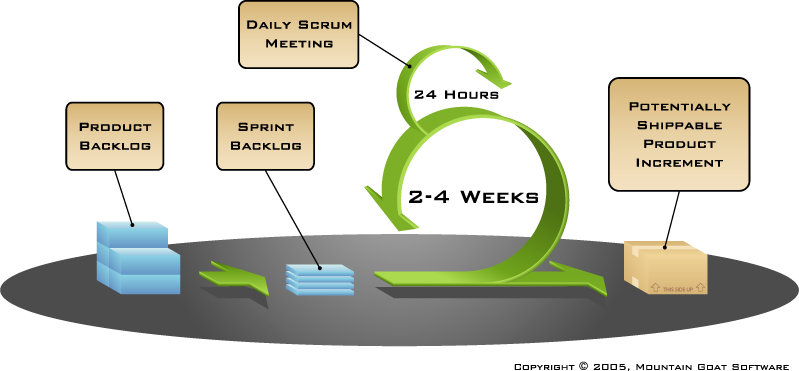
\includegraphics[width=1.0\textwidth]{Scrum.png}
\caption[Scrum-Organisation]{Schematische Organisation eines Projektes mit der Scrum-Methode\protect\footnotemark}
\label{fig:Scrum}
\end{figure}
\footnotetext{Quelle: \url{www.fossa.de}}

Das dargestellte Modell zeigt, dass der Projektinhalt zerteilt und in iterativen Schritten erarbeitet wird. Dieses
Vorgehen schafft, durch die Teilung in zwei iterative Teilprozesse, die nötige Flexibilität der Projektorganisation.
Zum einen ist im Scrum-Modell ein Bearbeitungsprozess vorgesehen
der in zwei bis vier Wochen durchlaufen wird. Dieses Zeitintervall wurde im vorliegenden Projekt für die Erreichung des
nächsten Meilensteins\footnotemark\ vorgesehen. Zum anderen ist ein kleineres Zeitintervall von einem Tag dargestellt, das
genutzt wurde, um kleinere Teilaufgaben auf dem Weg zum nächsten Meilenstein fertig zu stellen.

\footnotetext{Meilensteine stellen elementare Stationen im Verlauf des Projektes dar. Eine genauere Beschreibung
folgt im weiteren Verlauf.}

Durch die Scrum-Organisation konnten kleine Teilaufgaben dezentral bearbeitet werden, ohne die zentrale Erreichung des
nächsten Meilensteins aus den Augen zu verlieren. Eine Projektorganisation, die die aufgezeigten Anforderungen
erfüllt, ist damit definiert.

% \subsubsection*{Möglichkeiten der Projektorganisation}
% \label{sec:MoeglichkeitenProjektorganisation}

% % Scrum ist eine Methode der agilen Softwareentwicklung. Konkret stellt Scrum eine
% % agile Projektmanagementmethode dar. Eine solche Managementmethode behandelt
% % nicht die konkrete Struktur und Art der Zusammenarbeit im Team, sondern
% % beschränkt sich auf den Ablauf des Projektes. Bei einer Projektorganisation nach
% % der Scrum-Methode lassen sich grundsätzlich jeweils drei verschiedene Rollen,
% % Zeremonien und Artefakte unterscheiden. Diese sollen im Folgenden näher
% % beschrieben werden. Die drei zentralen Rollen der Scrum-Methode sind hierbei\ldots

% \subsubsection*{Planung der Projektorganisation}
% \label{sec:PlanungProjektorganisation}

% \subsubsection*{Umsetzung der Projektorganisation}
% \label{sec:UmsetzungProjektorganisation}

% Für eine erfolgreiche Durchführung des Projektes ist es unabdingbar sich vorher
% über die Projektorganisation im Klaren zu sein. Bei der Projektorganisation
% handelt es sich hierbei darum, wie die Entwicklung eines Projektes vonstatten
% gehen soll. Dies bedeutet, dass festgelegt wird, welche Entwicklungsmethodiken
% angewandt werden oder welche Hilfsmittel und Zusatztools eingesetzt werden, um
% das gewünschte Ziel des Projektes möglichst effizient zu erreichen. Ebenfalls
% umfasst dieser Aspekt den Punkt der Kommunikation und Interaktion des
% Projektteams und der einzelnen Projektmitglieder untereinander. Hinzu kommt,
% dass festgelegt wird, wie die einzelnen Meetings der Projektgruppe vonstatten
% gehen und welche Bedingungen erfüllt werden müssen.

% Bei dem großen Umfang und der Vielfalt dieses Projektes ist es notwendig
% flexibel zu sein und somit auf Probleme oder Änderungen und Wünsche des
% Auftraggebers zeitnah reagieren und umsetzen zu können. Um somit die
% Entwicklung agil zu gestalten, entschied man sich in diesem Projekt für die
% Scrum-Methode. Dies ist eine Methodik der agilen Softwareentwicklung und sorgt
% mit sogenannten Scrum-Meetings für regelmäßige Treffen der Projektmitglieder.
% Diese Scrum-Meetings werden immer in gleichen Abständen nach sogenannten
% Sprints gehalten. Die Sprints können hierbei 1 bis 30 Tage lang sein und
% stellen einzelne Iterationsschritte in der Entwicklung der Anwendung dar. Nach
% jeweils einem Sprint, entsteht eine weitere lauffähige Anwendung, aber um die
% Funktionen des letzten Sprints erweitert. Somit wird gewährleistet, dass immer
% eine lauffähige Version zur Verfügung steht und dem Auftraggeber vorgelegt
% werden kann. Nach Ablauf eines Sprints und des darauffolgenden
% Scrum-Meetings,werden weitere Arbeitspakete und Aufgaben an die einzelnen
% Projektmitglieder verteilt, welche in dem folgenden Sprint erledigt werden
% müssen. Durch die kurzen Sprints und häufigen Meetings können so Meinungen,
% Ideen und auch Probleme bei der Umsetzung unter den Projektmitgliedern
% diskutiert und beseitigt werden. Hierbei ist jedes Mitglied gleichberechtigt
% involviert. Trotz dessen können bei der Scrum-Methode folgende drei Rollen
% unterschieden werden:

% \begin{description}
% \item[Der Product Owner] stellt einen Vertreter für den Endkunden dar und
% vertritt somit dessen Wünsche und Bedürfnisse hinsichtlich der Anwendung. Der
% Product Owner trifft somit auch die Entscheidungen bzgl. Kosten und weiterer
% gewünschter Änderungen oder Vorgaben. Die Ergebnisse werden ebenfalls von
% diesem überprüft.
% \item[Der Scrum-Master] dient als Schnittstelle zwischen dem Product Owner und
% dem Scrum-Team und fördert die Zusammenarbeit. Ebenfalls sorgt er dafür, dass
% das Scrum-Team nach den Regeln der Scrum-Methode arbeiten.
% \item[Das Scrum-Team] ist für die Entwicklung und Implementierung der
% gewünschten Anwendung zuständig. Es handelt eigenständig und organisiert somit
% sich und die Vorgehensweise in großem Maße selbst.
% \end{description}

% Ebenfalls zu erwähnen ist, dass ein Product-Backlog ein vom Endkunden
% definierter Katalog ist, welcher die Anforderungen des Kunden , nach Priorität
% und Wichtigkeit sortiert, enthält. Die Anforderungen des Product-Backlog werden
% dabei in ein sogenanntes Sprint-Backlog übertragen, welches bei den Sprints als
% Vorlage für die zu erfüllenden Aufgaben dient. Nach jedem Sprint werden die
% erzielten Ergebnisse, unabhängig von der erreichten Vorgaben, in einem Sprint
% Review dokumentiert und an den Product Owner zur Einsicht übergeben.

% In folgender Abbildung wird der Scrum-Prozess nochmals visuell dargestellt:

% Nach einer kurzen Einführung in die agile Softwareentwicklung kann nun gesagt
% werden, dass das Projektteam in diesem Projekt agil entwickelt hat. Dazu wurde
% eine Sprintdauer von einer Woche angesetzt. Nach dieser Woche fand immer ein
% Scrum-Meeting statt, in der die Erkenntnisse und Ergebnisse der einzelnen
% Projektmitglieder reflektiert wurden. Für die einzelnen Scrum-Meetings sind
% ebenfalls Gesprächsprotokolle erstellt worden, auf die im Nachhinein
% zugegriffen werden kann (siehe Anhang). Bei besonders komplexen Problemen
% während der Entwicklung der Anwendung, wurde auf die Methode des Pair
% Programming zurückgegriffen. Dies bedeutet, dass mehrere Mitglieder
% gleichzeitig und zusammen an einem Rechner an einem Implementierungsproblem
% arbeiten. Dadurch konnten komplexe Probleme schneller und effizienter beseitigt
% werden, da sich die Teammitglieder während des Arbeitens direkt austauschen
% können. Zum Schluss jedes Scrum-Meetings wurden ebenfalls neue Arbeitspakete an
% die Gruppenmitglieder verteilt.

% Die Verwaltung der Arbeitspakete wurde dabei durch ein zusätzliches Tool
% realisiert, welches sich PHProjekt nennt. Dieses Tool ist ein webbasiertes
% Ticketsystem, welches es ermöglicht Arbeitspakete einzelnen Gruppenmitgliedern
% zuzuweisen und deren einzelne Status anzeigen zu lassen. Ebenfalls ist es hier
% möglich Prioritäten und Dauer zu definieren, um die wichtigsten Arbeitspakete
% zu kennzeichnen und eine Frist zur Erledigung zu setzen.

% Um die einzelnen Programmversionen, welche nach den Sprints entstehen, zu
% verwalten, wurde die Versionsverwaltung Github eingesetzt, welche ebenfalls
% webbasiert arbeitet. Hiermit ist es möglich Abspaltungen von einer bestehenden
% Programmversion zu erzeugen und diese zu bearbeiten und nach Abschluss wieder
% der Stammversion hinzuzufügen. So kann gewährleistet werden, dass immer eine
% funktionsfähige Version zur Verfügung steht, da isoliert von der Stammversion
% gearbeitet und entwickelt wird.
\subsection{Projektphasen}
\label{sec:Projektphasen}

Nachdem im vorherigen Abschnitt die Organisation des Projektes erläutert wurde,
wird im Folgenden das Projekt in Phasen gegliedert. Die Phasen dienen 
dazu, das Projekt in einem geordneten Ablauf zu strukturieren und
Arbeitsschritte aufeinander aufbauend zu vergeben. "`Der Aufbau der
Projektphasen ist darauf ausgerichtet, systematisch und aufeinander aufbauend
zu 'lernen', um insgesamt eine optimale Entscheidungsprozedur zu
durchlaufen"'.\footnote{\citet{walter2006}}

Jede Projektphase stellt dabei eine in sich geschlossene Einheit dar, die aus
mehreren Arbeitspaketen und Meilensteinen bestehen kann. Arbeitspakete sind
dabei konkrete Arbeitsschritte, die von einer ausgewählten Person in einem
gewählten Zeitraum zu erfüllen sind. Jedes Arbeitspaket arbeitet auf die
Erfüllung des jeweils nächsten Meilensteines hin.

Meilensteine bilden wichtige, elementare "`Stationen"' in einem Projekt ab. Sie
strukturieren das Projekt durch zeitliches Festlegen von Teilzielen.
Darüber hinaus kann an den abgeschlossenen Meilensteinen
der Erfüllungsgrad des Projektzieles abgelesen werden.\footnote{\citet{schels2008}}

Jede Projektphase endet daher mit einem Meilenstein. Der Projektphasenplan mit
den jeweiligen abschließenden Meilensteinen ist in nachfolgender Abbildung
dargestellt:

\begin{figure}[htb] 
\centering
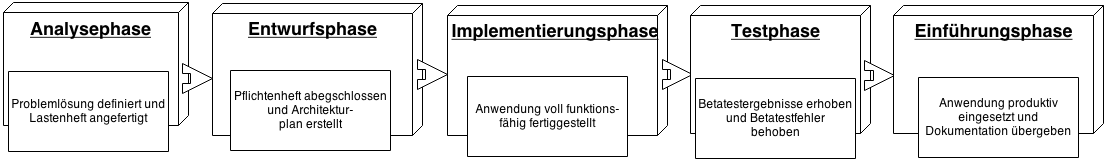
\includegraphics[width=1.0\textwidth]{Phasenplan.png}
\caption[Phasenplan des Projektes]{Phasenplan des Projektes\protect\footnotemark}
\label{fig:MockupFrontend}
\end{figure}
\footnotetext{eigene Darstellung}

\begin{description}

  \item[Die Analysephase] ist Ausgangspunkt der vorliegenden Projektarbeit. Sie setzt
  auf der aktuellen Ist-Situation an und in ihr werden Lösungsmöglichkeiten für
  das vorhandene Problem analysiert. Am Ende der Analysephase steht eine
  konzeptionelle Problemlösung. Das bedeutet konkret, aus der Analyse der
  vorliegenden Situation werden verschiedene Lösungsansätze entwickelt. Im
  Zuge der Analyse und Auswertung dieser Lösungsansätze wird ein Ansatz
  ausgewählt, der für die Lösung am geeignetsten ist. Die Analysephase ist in
  der vorliegenden Ausarbeitung im \verweis{Konzeptionierung} beschrieben.

  Die Ergebnisse der Analyse werden in einem Lastenheft\footnote{\citet{lastenheft2013}} formuliert.

  Die Analysephase wird mit dem Meilenstein "`Problemlösung definieren und
  Lastenheft angefertigt"' abgeschlossen.

  \item[Die Entwurfsphase] folgt im Anschluss auf die Analysephase.
  Ausgangspunkt der Entwurfsphase ist ein angefertigtes Lastenheft. Aufgrund der
  darin beschriebenen Anforderungen kann die Planung der Umsetzung
  begonnen werden. Die
  Entwurfsphase beinhaltet dabei Modelle und Entwürfe, 
  die konkret beschreiben, wie die
  Anforderungen des Lastenheftes umgesetzt werden. Das Ergebnis der Entwurfsphase ist ein erstelltes Pflichtenheft, das die konkretisierte Umsetzung des Problems
  beschreibt.

  Im vorliegenden Projekt wurden systematisch verschiedene Teilgebiete der
  entstehenden Lösung betrachtet und mit Modellen individuell konzipiert, um die
  Komplexität einer solchen Lösung in kleinere Teilbereiche zu unterteilen. Dabei
  wurden hauptsächlich die Bereiche Datenhaltung bzw. Datenbankdesign und
  Anwendungslogik voneinander getrennt betrachtet. Dieser getrennten Betrachtung
  ging dabei der Entwurf eines ersten Oberflächendesigns, ein sogenanntes
  Mockup, voraus. Mit diesem Mockup konnte ein erster Eindruck über Umfang und
  Komplexität gewonnen und zusätzlich Funktionalität und Benutzung
  verdeutlicht werden. Eine Abbildung dieses Mockups ist an Anhang ~\ref{sec:Mockup} zu sehen.

  Eine genauere Betrachtung der Entwurfsphase würde an dieser Stelle zu weit führen,
  kann aber in \citet{modelierungUndBetrieb2014} nachgelesen werden.
  Das angefertigte Pflichtenheft kann in \citet{pflichtenheft2013} nachgelesen werden.

  Die Entwurfsphase wurde mit dem Meilenstein "`Pflichtenheft abgeschlossen und
  Architekturplan erstellt"' abgeschlossen.

  \item[Die Implementierungsphase] folgt im Anschluss an die Entwurfsphase und
  baut auf einem abgeschlossenen Pflichtenheft auf. Diese Phase ist sowohl die
  zeitlich größte Phase als auch die Entscheidende, da in dieser Phase alle im
  Vorfeld geplanten Schritte und Modelle umgesetzt werden. In der Phase der
  Implementierung werden, aufbauend auf den vorher angefertigten Entwürfen, die
  theoretischen Modelle in ausführbaren Quellcode umgesetzt. In dieser Phase
  zeigt sich vor allem die Qualität der angefertigten Modelle, denn am
  schnellsten lässt sich Software entwickeln, wenn das dazugehörige Modell
  1:1 in Quellcode übertragen werden kann. Allerdings ist das, aufgrund der
  Schwierigkeit eine Software in seiner Komplexität in einem Modell zu erfassen,
  häufig schwer zu erreichen. Bei unerwartetem Abweichen vom Modell muss daher
  die Konzeption der Software erneut überdacht werden, um eventuellen logischen
  Fehlern vorzubeugen. Der Prozess dieser Implementierung kann in der
  Ausarbeitung Modellierung und Betrieb in Kapitel 5. (Umsetzung) nachgelesen werden.

  Die Implementierungsphase endet mit dem Meilenstein "`Anwendung voll
  funktionsfähig fertiggestellt"'.

  \item[Die Testphase] baut auf der fertigestellten und funktionierenden Software auf.
  Idealerweise wird der Test der Software von Personen durchgeführt, die nicht im Prozess der
  Softwareentwicklung beteiligt waren. Diese Personen haben eine
  unbeeinflusste Sicht auf die Software. Sie können so zum einen dessen
  intuitive Bedienung besser einschätzen und zum anderen benutzen sie die Software auch
  unvoreingenommen.Dies kann dazu führen, das sie Fehler in der Bedienung oder
  im Programm entdecken.Einen solchen Test, der von außenstehenden Personen
  durchgeführt wird, wird als Betatest bezeichnet. Diesem Betatest ist im
  Idealfall ein Alphatest der Entwickler vorausgegangen, in dem sie die entwickelten Anwendungsfälle (use cases) im fertigen Programm simulieren und dabei mögliche
  Fehler entdecken und ausbessern können. Der Alphatest wird in dieser Ausarbeitung nicht näher betrachtet,
  kann aber in \citet{modelierungUndBetrieb2014} nachgelesen werden.
  In der Betatestphase ist es besonders wichtig die  aufgetretenen Fehler
  und Kritiken zu erfassen und an die Entwickler weiterzugeben. Durch den
  Betatest können sogenannte "`Kinderkrankheiten"' früh erkannt und beseitigt
  werden. Das steigert die Qualität und erhöht vor allem die
  Benutzerzufriedenheit beim verwenden der Software. Die Betatestphase wird zudem im Folgenden
  zur Verifizierung von Projektzielen verwendet.\footnote{siehe \verweis{Zielkatalog}}

  Die Testphase wird mit dem Meilenstein "`Betatestergebnisse erhoben und
  Betatestfehler behoben"' abgeschlossen.

  \item[Die Einführungsphase] erfolgt nach erfolgreicher Fertigstellung der Software und Korrektur aller
  aufgetretenen Fehler. Die Software wird in dieser Phase dem Auftraggeber übergeben und produktiv eingesetzt.
  Zur Übergabe der Software gehört zudem eine Dokumentation der Funktionsweise, die im \verweis{Anwenderdokumentation} vorgestellt wird. Der Abschluss dieser Phase stellt damit den Abschluss des Projektes dar.

  Die Einführungsphase endet mit dem letzten Meilenstein "`Anwendung produktiv
  eingesetzt und Dokumentation übergeben"'.

\end{description}
\subsection{Projektrealisierung}
\label{sec:Projektrealisierung}

Aufbauend auf der Festlegung der Projektphasen kann das Projekt iterativ anhand der aufgezeigten Organisation
realisiert werden. An dieser Stelle setzt die konkrete Beschreibung der Realiesierung des
Projektes in \citet{modelierungUndBetrieb2014} an.
Ein Einblick in diese Realesierung wäre an dieser Stelle zu umfassend und zu komplex. Aus diesem Grund werden an dieser
Stelle nur die Ergebnisse der Projektrealsierung vorgestellt.

Realisiert werden sollte eine visuelle Ansicht des neuen Campus Lingen, in dem sich der Benutzer im Stile von Google
Street View frei umsehen kann. Diese Realiserung ist gelungen und das Eregbnis ist in \abbildung{FrontendFinal}
zu sehen:

\clearpage

\begin{figure}[htb] 
\centering
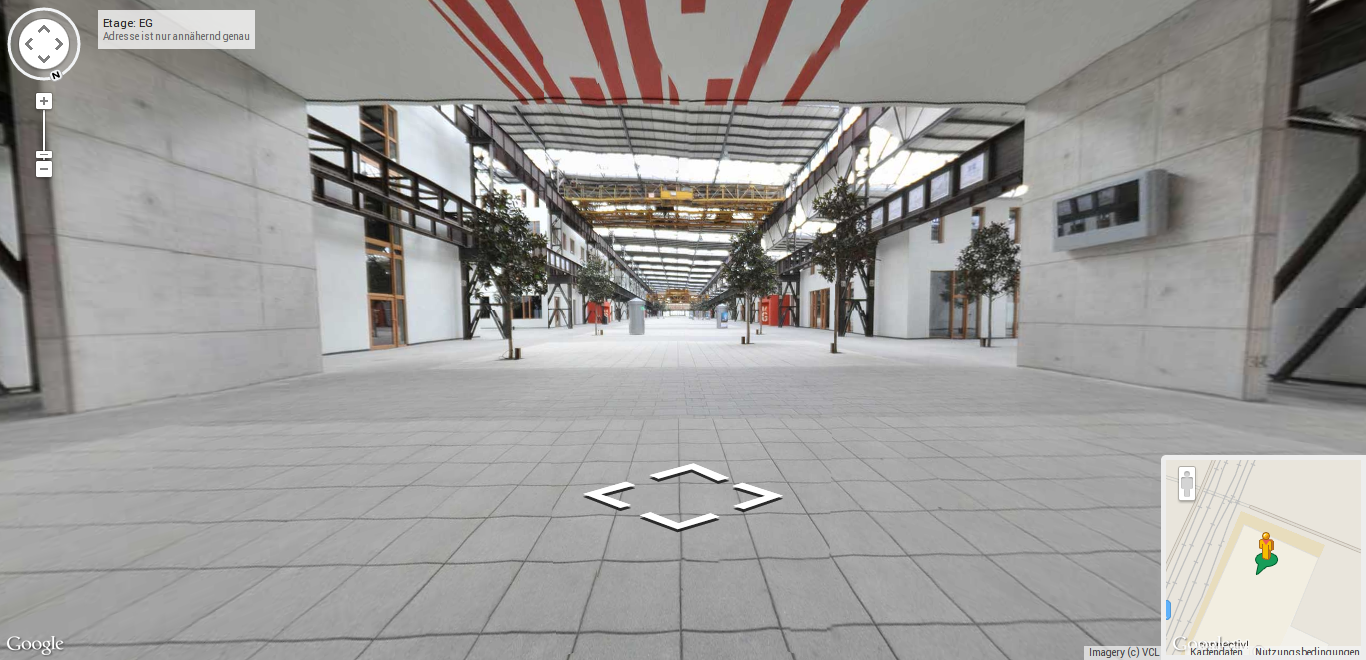
\includegraphics[width=1.0\textwidth]{FrontendFinal.png}
\caption[Abbildung der Benutzeransicht]{Ein Bildschirmfoto der fertigen Benutzeransicht\protect}
\label{fig:FrontendFinal}
\end{figure}

Neben dieser Benutzeransicht sollte darüber hinaus vor allem die Nachhaltigkeit des Projektes gewahrt werden.
Hierzu sollte ein Administrationsbereich entwickelt werden, in dem es möglich ist alle Informationen
der Benutzeransicht zu pflegen. Ein Ausschnit dieses Administrationsbereiches ist 
in \abbildung{BackendFinal} dargestellt:

\begin{figure}[htb] 
\centering
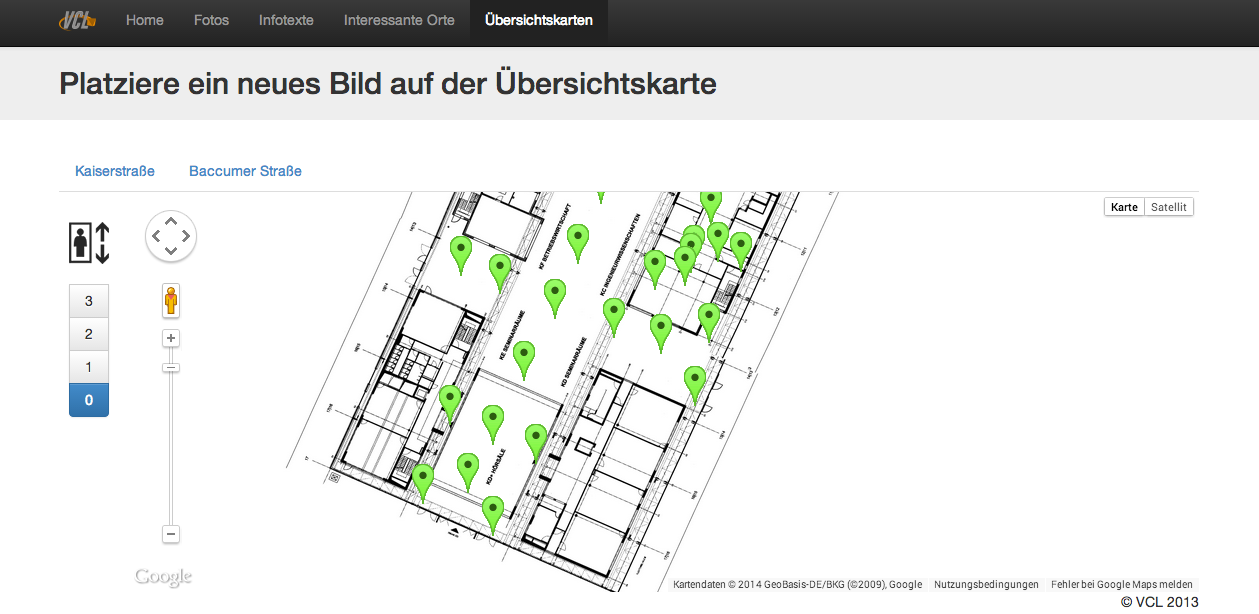
\includegraphics[width=1.0\textwidth]{BackendFinal.png}
\caption[Ausschnitt des Administrationsbereiches]{Verwalten und Platzieren von Panoramafotos im Administrationsbereich\protect}
\label{fig:BackendFinal}
\end{figure}
\subsection{Projekttest}
\label{sec:Projekttest}

Der Projekttest dient im vorliegenden Projekt zur Verifikation der beschriebenen
Projektziele und zur Behebung von Fehlern innerhalb der Anwendung. Der
Projekttest gliedert sich dabei in zwei aufeinander folgende Phasen. In der
ersten Phase wird das Projekt vom Entwicklerteam selbst, anhand von erstellten
Anwendungsfällen, getestet. Einen solchen Test bezeichnet man als Alphatest, da
dieser von Personen durchgeführt wird, die an der Entwicklung beteiligt waren.
Der Alphatest dient primär zur Erkennung und Beseitigung von Fehlern in der
Anwendung. Der Abschluss dieses Test verifiziert, dass die Anwendung fehlerfrei
funktioniert. Aufbauend auf dem Alphatest wird ein Betatest der Anwendung von
aussenstehenden Personen durchgeführt. Dieser Test dient primär zur
Verifizierung der Projektziele. Der Alphatest wird an dieser Stelle nicht weiter
vertieft, da dieser für die Betrachtung des vorliegenden Themenbereiches nicht
relevant ist. Die Durchführung und Ergbnisse können in
\citet{modelierungUndBetrieb2014} im Kapitel 6 (Test) nachgelesen werden. Der
Fokus des Projekttests liegt im Folgenden auf dem durchgeführten Betatest.

Zur Durchführung des Betatests wurde im ersten Schritt ein definierter Bereich
des Campus in die erstellte Anwendung eingepflegt. Dieser Bereich zeigt den
Betatestern einen repräsentativen Ausschnitt des Campus.
Im zweiten Schritt wurde ein Onlinefragebogen vorbereitet, der von Betatestern
nach Benutzung der Anwendung ausgefüllt werden soll. Dieser Fragebogen enthält 
sowohl Fragen, die der Verifizierung der Zielerreichung dienen, als auch
Fragen, die dem Entwicklerteam Auskunft über mögliche Schwachstellen des Systems geben.
Da an dieser Stelle nur der Teil der Fragen, der zur Verifikation der Ziele dient,
interessant ist, wird nur ein Auschnitt des gesamten Fragebogens in\tabelle{Fragebogen} dargestellt.

An dem Betatest haben insgesamt 97 Personen teilgenommen. Die Auswertung der Tests ist in nachfolgender Tabelle
festgehalten:

\clearpage
\tabelleEinfg{Auswertung des Betatests}{tab:Fragebogen}{AuswertungBetatest}

Aufbauend auf diesen Ergebnissen erfolgt die Verifikation der Zielerreichung in \verweis{Zielerreichung}.
Der subjektive Eindruck der Betatester, der in obiger Tabelle in der letzten Spalte abzulesen ist,
zeigt dem Entwicklerteam aber bereits eine erste positive Resonanz.
\subsection{Anwenderdokumentation}
\label{sec:Anwenderdokumentation}

Zur Gewährleistung der Nachhaltigkeit ist es Ziel des Projektes eine
Dokumentation zu erstellen, die die Administrations- und Pflegefunktionen der
Anwendung erläutern. Der grobe Inhalt dieser Dokumentation wird im Folgenden
kurz vorgestellt, um einen Überblick über die Pflege der Anwendung zu geben. Die
vollständige Version kann in \citet{projektdokumentation2014} nachglesen werden.

Die Dokumentation umfasst die folgenden Teilbereiche:

\begin{itemize}
  \item Hinzufügen und Ändern von Fotos
  \item Hinzufügen und Ändern von Infotexten
  \item Hinzufügen und Ändern von interessanten Orten
  \item Positionieren von Fotos
  \item Zuordnung von Infotexten und Fotos
  \item Festlegen von Nachbarschaftsbeziehungen zwischen Fotos
\end{itemize}

Bei Pflege der Anwendung müssen in erster Linie Fotos, Infotexte und interessante Orte gepflegt werden. Die \textbf{Fotos}
sind dabei das Basiselement der Anwendung. Hier müssen Panoramabilder angefertigt und in kleinere Bildteile zerschnitten
werden. Die Hintergründe zu dieser Vorgehensweise werden in \citet{modelierungUndBetrieb2014} im
Kapitel 5.1 (Panoramaerstellung) beschrieben.
Die \textbf{Infotexte} dienen zum Anzeigen von relevanten Informationen auf einem Foto. In Infotexten können
zum Beispiel Projekte vorgestellt oder Öffnungszeiten von Gebäuden angezeigt werden. Die gesamte Informationsvermittlung
findet im Projekt über Infotexte statt.
Zum Navigieren durch den Campus stehen dem Benutzer zum einen die Navigationspfeile und zum anderen die
\textbf{interessanten Orte} zur Verfügung. Dem Benutzer wird durch Klick auf die
Übersichtskarte eine Liste mit Orten angezeigt, zu denen er springen kann.
Diese Navigationsmöglichkeit hilft Studieninteressierten schnell Orte, wie die
Bibliothek oder das Fachbereichsgebäude zu finden, ohne dass sie diese suchen
müssen. Diese interessanten Orte müssen aber im Administrationsbereich der
Anwendung hinterlegt und gepflegt werden.

Aufbauend auf der Pflege dieser Grundinformationen müssen in der Anwendung noch
weiterführende Zusatzinformationen gepflegt werden. Dazu zählt zum einem das
Positionieren des Fotos auf einer topographischen Karte, die Zuordnung zu
Infotexten und das Festlegen von Nachbarschaftsbeziehungen. Ist ein Foto
positioniert, kann es dem Benutzer im Frontend angezeigt werden. 
Sollen auf diesem Foto zusäzlich ein oder mehrere Infotexte angezeigt werden,
müssen die entsprechende Infotexte an das Foto angehängt werden. Diese Zuordnung
wird im Administrationsbereich gepflegt. Ebenso wird die angesprochene
Navigation zwischen zwei Fotos über die Navigationspfeile im
Administrationsbereich gepflegt. Dazu müssen zu jedem hochgeladenen und
positionierten Foto Nachbarfotos definiert werden. Diese Nachbarfotos werden dem
Benutzer als Navigationspfeile angezeigt.

\subsection{Projektabschluss}
\label{sec:Projektabschluss}

Das Projekt Virtueller Campus Lingen ist mit abschließender Fertigstellung der Anwenderdokumentation
abgeschlossen. Das Projekt muss in dieser Projektphase dem Auftraggeber übergeben werden.
Das zu übergebende Projekt besteht dabei aus den folgenden Teilen:

\begin{itemize}
  \item den vollständigen Quellcode der Software
  \item eine Kopie der Datenbank nach Abschluss des Projektes (Sicherheitskopie)
  \item die Installation der Webanwendung auf einem Webserver
  \item die Internetadresse der Anwendung und alle benötigten Passwörter
  \item eine Einführung in die Verwendung der Software anhand der Dokumentation
\end{itemize}

Auf Basis dieser Informationen und Materialien ist der Auftraggeber in der Lage das Projekt zu pflegen und zu erweitern. Die Wahrung der Nachhaltigkeit ist damit vollständig gewährleistet. Die Installation und Übergabe der Webanwendung ist für Mitte Juli 2014 geplant.
\section{Projektreflexion}
\label{sec:Projektreflexion}

In Nachfolgender Betrachtung werden die geplanten Projektressourcen reflektiert und mit aufgenommen Ist-Daten verglichen.
Dem Projektauftraggeber wird im Folgendem ein abschließender Überblick über Zeit- und Kostenaufwand des Projektes gegeben.
Weiterführend wird die Zielerreichung reflektiert und der Grad der Zielerreichung bestimmt. Auf dieser Basis kann der
enstandene Aufwand dem erhaltenen Nutzen gegenübergestellt werden.

\subsection{Zeitmanagement}
\label{sec:Zeitmanagement}

Aus dem \verweis{TerminplanungUndZeitManagement} ist zu entnehmen, dass 760 Stunden Arbeitsaufwand für das Projekt
eingeplant wurden. Das Gantt-Diagramm in Abbildung XX zeigt, dass tatsächlich
ein Aufwand von 987 Stunden enstanden ist.
% TODO: Abbildung XX fürs Gantt Diagramm richtig einfügen.
Die Differenz dieses Arbeitsaufwandes wird in \tabelle{SollIstVergleichZeit} differenzierter dargestellt.

\begin{table}[h]
\centering
\begin{tabular}{ccccl}
\hline
\multicolumn{1}{l}{}                 & Plan {[}h{]} & Ist {[}h{]} & Differenz {[}h{]} & Differenz {[}\%{]} \\ \hline
Foto aufnehmen                       & 20           & 30          & +10               & + 50,00\%          \\ \hline
Fotos aufbereiten                    & 10           & 60          & +50               & +500,00\%          \\ \hline
Organisation                         & 37           & 29          & -8                & -21,62\%           \\ \hline
Implementierung Benutzerbereich       & 120          & 100         & -20             & -16,67\%           \\ \hline 
Implementierung Administrationsbereich & 314         & 485 & +171              & +54,46\%           \\ \hline 
Umsetzung Vor- und Nachbereitung     & 129          & 166         & +37               & +28,68\%           \\ \hline
Sonstiges                            & 130          & 117         & -13               & -10,00\%           \\ \hline
                                     & 760          & 987         & +227              & +29,87\%           \\ \hline
\end{tabular}
\caption{Soll-Ist-Vergleich der Zeitplanung}%
\label{tab:SollIstVergleichZeit}%
\end{table}


Der Mehraufwand von 227 Stunden ist vorallem durch Abweichungen in der Implementierung des Administrationsbereiches
enstanden. Dieser Teilbereich des Projektes verursachte einen Mehraufwand von
171 Stunden, der vor allem darauf zurückzuführen ist, dass die Implementierungslogik in diesem Bereich oft überarbeitet werden musste.

Darüber hinaus ist zu erkennen, dass in Relation zu dem geplanten Aufwand die Aufbereitung der Fotos die Größte
prozentuale Differenz aufweist. Der Aufwand dieses Arbeitsbereiches wurde zu Beginn des Projektes unterschätzt.
Der Fotobearbeitungsprozess wurde innerhalb der Projektentwicklung ständig verfeinert und stellt am Ende des Projekts
einen komplexen eigenständigen Prozess dar. Die Vertiefung dieser Prozesskomplexität würde an dieser Stelle zu weit
führen, ist aber in \citet{modelierungUndBetrieb2014} im Kapitel 5.1 (Panoramaerstellung) dokumentiert.
\subsection{Kostenmanagement}
\label{sec:Kostenmanagement}

% Was war Kostentechnisch geplant?
% Was ist der tatsächlich ist Zustand
% Woran kann man das festmachen?
% Warum ist das so?

Die Kostenplanung in \verweis{Kostenplanung} zeigt, dass keine Kosten für die Entwicklung des vorliegenden Projektes
geplant waren. Im Verlauf des Projektes konnte wie geplant das gesamte Equipment selbst gestellt oder geliehen werden,
sodass keine realen Kosten im Projekt angefallen sind. Der Kostenplan wurde eingehalten.

Im vorherigen \verweis{Zeitmanagement} wurde aber bereits aufgezeigt, dass der Zeitaufwand nicht der Planung entsprach und
dieser Zeitaufwand beeinflusst das Kostenmanagement. Praktisch fallen zwar keine Personalkosten für das vorliegende Projekt
an, aber sie werden aus zu statistischen Zwecken für den Auftragegeber und zur
Wertbestimmung des Projekt trotzdem berücksichtigt. Im vorherigen Abschnitt wurde ein zeitlicher Mehraufwand von \textbf{227} Stunden festgestellt. Dieser
wird mit einem statistischen Kostensatz von 60€/Stunde berechnet. Daraus ergibt sich folgende dargestellte
Auswirkung auf das Kostenmanagement:

\tabelleEinfg{Soll-Ist-Vergleich der Kostenplanung}{tab:SollIstVergleichKosten}{KostenVergleich}

Es ergeben sich statistische personelle Mehrkosten von \textbf{13.620€}. Die Kosten
für die Weiterführung des Projektes belaufen sich auf \textbf{2.763}. Der abschließende
über die Kosten definierte Projektwert beläuft sich damit auf \textbf{61.983€}.

Es müssten damit nur \textbf{4,46\%} des Projektwertes vom Auftraggeber investiert werden,
um das Projekt zu erhalten und die Ziele dieses zu nutzen.
\subsection{Zielerreichung}
\label{sec:Zielerreichung}

Die zu erreicheneden Ziele des Projekts wurden in \verweis{Zielkatalog} aufgestellt und erläutert. Im Folgenden
wird ermittelt, ob und in welchem Ausmaß diese Ziele erreicht werden konnten.
Aus den erreichten Zielen kann darauf folgend der Nutzen der Anwendung für die Auftraggeber verifiziert werden.

Die Verifizierung der Zielerreichung wird dabei in zwei Teilschritten vollzogen. Im ersten Schritt werden alle
Ziele untersucht, deren Erfolg von der Projektgruppe selbst verifiziert werden kann. Im Anschluss daran werden
die Teilziele untersucht, deren Erfolg durch Dritte (z.B. durch den Fragebogen im Betatest) verifiziert wird.

Die folgende Aufstellung listet im ersten Schritt alle Ziele mit dem entsprechenden Grad der Zielerreichung auf,
die von der Projektgruppe selbst verifiziert werden können.

\begin{table}[h]
\centering
\begin{tabular}{ccccl}
\hline
\multicolumn{1}{l}{}                 & Zielkategorie & Zielindikator & Grad der Zielerreichung &              \\ \hline
Abbildung aller Institute                 & Muss-Ziel     & Anzahl Bilder pro Institut > 10   & 100\%   \\ \hline
Aufbau einer Administrationsoberfläche    & Muss-Ziel     & Möglchkeit der Pflege             & 100\%   \\ \hline
Entwicklung einer Anwenderdokumentation   & Muss-Ziel     & Anwenderdokumentation vorhanden   & 100\%   \\ \hline
Einhaltung der Datenschutzrichtlinien     & Muss-Ziel     & Keine Abweichungen                & 100\%   \\ \hline
Einhaltung der IT-Sicherheit              & Muss-Ziel     & Kein Eindringen möglich           & 100\%   \\ \hline
Alleinstellungsmerkmal erzielen           & Soll-Ziel     & Vergleich zu anderen Hochschulen  & 100\%   \\ \hline
Geringe Betriebskosten erzielen           & Soll-Ziel     & Hostinggebühren < 20€             & 100\%   \\ \hline
Geringe Entwicklungskosten erzielen       & Soll-Ziel     & tatsächliche Entwicklungskosten < 100€  & 100\%   \\ \hline
\end{tabular}
\caption{Zielerreichung der selbstverifizierten Ziele}%
\label{tab:Zielerreichung1}%
\end{table}

Aus der dargestellten Auflistung ist zu entnehmen, dass im ersten Schritt alle Ziele erreicht werden konnten.
Dem Auftraggeber kann damit verifizert werden, dass die entwickelte Anwendung ein zukunftsorientertes Projekt mit
Alleinstellungscharakter ist.

In einem zweiten Schritt verifizieren die Antworten der Betatester die Erreichung weiterer Ziele:


% \begin{table}[h]
% \centering
% \begin{tabular}{ccccl}
% \hline
% \multicolumn{1}{l}{}                 & Zielkategorie    & Zielindikator & erreichter Wert & Grad der Zielerreichung &              \\ \hline
% Steigerung der Attraktivität              & Muss-Ziel   & Frage Nr. XX mind 3,0                   & 100\%   \\ \hline
% Aufbau einer Administrationsoberfläche    & Muss-Ziel     & Möglchkeit der Pflege             & 100\%   \\ \hline
% Entwicklung einer Anwenderdokumentation   & Muss-Ziel     & Anwenderdokumentation vorhanden   & 100\%   \\ \hline
% Einhaltung der Datenschutzrichtlinien     & Muss-Ziel     & Keine Abweichungen                & 100\%   \\ \hline
% Einhaltung der IT-Sicherheit              & Muss-Ziel     & Kein Eindringen möglich           & 100\%   \\ \hline
% Alleinstellungsmerkmal erzielen           & Soll-Ziel     & Vergleich zu anderen Hochschulen  & 100\%   \\ \hline
% Geringe Betriebskosten erzielen           & Soll-Ziel     & Hostinggebühren < 20€             & 100\%   \\ \hline
% Geringe Entwicklungskosten erzielen       & Soll-Ziel     & tatsächliche Entwicklungskosten < 100€  & 100\%   \\ \hline
% \end{tabular}
% \caption{Zielerreichung der selbstverifizierten Ziele}%
% \label{tab:Zielerreichung1}%
% \end{table}



\subsection{Subjektive Reflexion}
\label{sec:SubjektiveReflexion}
\section{Ausblick}
\label{sec:Ausblick}

Am Ende des Projektes sollen an dieser Stelle Ideen und Anregungen zur Weiterführung des Projektes gegeben werden. Viele dieser Ideen kamen während des Projektverlaufes auf, ließen sich aber aus zeitlichen Gründen nicht realisieren.

Ein Beispiel dafür ist die Umsetzung einer geführten Tour für Studieninteressierte durch bestimmte Studienbereiche. Auf Messen wäre es dadurch möglich Auschnitte und Informationen zu bestimmten Studienbereichen ohne Benutzerinteraktion zu zeigen. Auch für Studieninteressierte, die sich nicht selbst durch den Campus bewegen, sondern lediglich die wichtigsten Informationen zu Ihrem Studiengang erhalten wollen, wäre dieser Ansatz interessant.

Gleichzeitig wäre besonders bei den erwähnten Messeauftritten eine Version der Software von Vorteil, die ohne Internetanbindung verwendet werden kann. Zum Zeitpunkt des Projektabschlusses greift die Software auf einige Programmbibliotheken (vor allem im Javascript Bereich) übers Internet zu. Diese Zugriffe könnten auch offline erfolgen, wenn man die Bilbiotheken runterlädt und lokal einbindet. Die teure Internetanbindung auf Messen, wenn überhaupt eine vorhanden ist, könnte dadurch vermieden werden.

Darüber hinaus gab es auch Ideen den Campus und seine Darstellung durch besondere Aufnahmen, zum Beispiel bei Nacht, noch einzigartiger zu gestalten. Es wäre denkbar Panoramafotos bei Nacht zu erstellen und in die bestehende Anwendung einen "`Nachtmodus"' zu implementieren, der vom Benutzer über einen Schalter ausgewählt werden könnte. Der Kreativität sind an dieser Stelle keine Grenzen gesetzt.
\section{Handlungsempfehlung}
\label{sec:Handlungsempfehlung}

Nach Abschluss des Projektes \ac{VCL} ist es für den Auftraggeber wichtig zu wissen,
ob das vorliegende Projekt eingeführt und weitergeführt werden sollte.
Hierzu wurden in der vorliegenden Ausarbeitung die wichtigsten Kennzahlen des Projektes,
einschließlich der anfallenden Kosten und der verifizierten Ziele, vorgestellt.
Diese Kosten sollen an dieser Stelle noch einmal kurz revidiert werden:

Die Weiterführung des Projektes kostet den Auftraggeber \textbf{2.763 €}, wobei
die erstellte Anwendung im Rahmen einer Unternehmensleistung, bedingt
durch Personal- und Materialkosten, ca. \textbf{61.983 €} kosten würde.
Der Auftraggeber hat damit einen Kostenvorteil von \textbf{95,54\%}.

Dieser Kostenvorteil rentiert sich für den Auftraggeber aber nur, wenn
das Projekt auch einen entsprechenden Mehrwehrt liefert.
Dem Auftraggeber wurde dazu nachweisbar in der vorliegenden Ausarbeitung aufgezeigt,
dass das die Ausendarstellung des Campus verbessert, eine junge Zielgruppe
von studieninteressierten direkt angesprochen wird und dabei noch für
Nachhaltigkeit und Innovativität gesorgt ist. Zudem hat keine andere
Hochschule eine solche Präsentation des eigenen Campus. Ein Alleinstellungsmerkmal
kann definitv erreicht und die daraus resultierenden Marketingeffekte effektiv genutzt werden.

Die Entscheidung dieses Projekt unter diesen Bedingungen Einzuführen
bleibt dabei dem Auftraggeber vorbehalten. Eine Empfehlung dafür wird an dieser
Stelle jedoch seitens der Autoren ausgesprochen. Darüber hinaus empfehelen die
Autoren den Erhalt und die Weiterführung dieses Projektes mit den vorgestellten Möglichkeiten.